\documentclass{report}
\usepackage[margin=1in, paperwidth=8.5in, paperheight=11in]{geometry}
%Math packages%
\usepackage{amsmath}
\usepackage{amsthm}
%Spacing%
\usepackage{setspace}
\onehalfspacing
%Lecture number%
\newcommand{\lectureNum}{5}
%Variables - Date and Course%
\newcommand{\curDate}{January 17, 2017}
\newcommand{\course}{CS 251}
\newcommand{\instructor}{Stephen Mann}
%Defining the example tag%
%\theoremstyle{definition}%
\newtheorem{ex}{Example}[section]
%Setting counter given the lecture number%
\setcounter{chapter}{\lectureNum{}}
%Package to insert code%
\usepackage{listings}
\usepackage{courier}
\usepackage{xcolor}
\lstset { %
    tabsize=2,
    breaklines=true,
    language=C++,
    backgroundcolor=\color{blue!8}, % set backgroundcolor
    basicstyle=\footnotesize\ttfamily,% basic font setting
}
%Package used to draw circuits%
\usepackage{circuitikz}
\begin{document}
%Note title%
\begin{center}
\begin{Large}
\textsc{\course{} | Lecture \lectureNum{}}
\end{Large}
\end{center} 
\noindent \textit{Bartosz Antczak} \hfill
\textit{Instructor: \instructor{}} \hfill
\textit{\curDate{}}
\rule{\textwidth}{0.4pt}
% Actual Notes%
\subsubsection{Review of Multiplexors}
A multiplexor takes in $n$ select lines, and $2^n$ inputs, and based on the value of the select lines, the multiplexor selects which input $D_i$ to output.
%TODO include table for 4-1 MUX and diagram from notes%
\section{RAM}
32 bits of memory isn't enough, so that's why we have \textit{Random Access Memory} (RAM). Static RAM (SRAM) uses D latches to store data. This memory is very slow compared to CPU speed; it's also not clocked.
\subsection{Three-state Buffers}
Has three outputs: 0, 1, and \textit{floating} (which means neither connected to power or ground). Uses a control (which can either be 1 or 0) to connect or disconnect data flow. When connected, the data is either 0 or 1 (obviously) and when it's disconnected, the data is floating (which means that there is not connection)
\begin{figure}[ht]
\begin{center}
        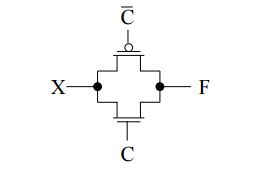
\includegraphics[scale=0.5]{tri_state_diagram.jpg}
\end{center}
\caption{The mechanics of a three-state buffer. If control ($C$) is 1, $F$ copies $X$ (i.e., there is a connection); otherwise, $F$ is floating (i.e., there is no connection). Courtesy of Prof. Mann's slides.}
\end{figure}\\
On notes and assignments, a three-state buffer is drawn as
\begin{figure}[ht]
\begin{center}
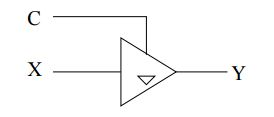
\includegraphics[scale=0.5]{tri_state_diagram2.jpg}
\end{center}
\caption{$C$ defines the control, and $X$ and $F$ are the input and output respectively. Courtesy of Prof. Mann's slides.}
\end{figure}
\newpage
\begin{ex}
An XOR from three-state buffers:
\end{ex}
\begin{figure}[ht]
\begin{center}
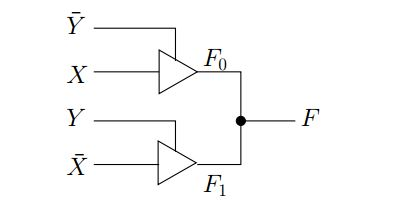
\includegraphics[scale=0.5]{tri_state_diagram3.jpg}
\end{center}
\caption{Courtesy of Prof. Mann's slides.}
\end{figure}
If we fill in the truth table for this diagram we have
\begin{center}
\begin{tabular}{ c c | c c | c c | c }
$X$ & $Y$ & $\bar{X}$ & $\bar{Y}$ & $F_0$ & $F_1$ & $F$ \\ \hline
0 & 0 & 1 & 1 & 0 & | & 0 \\
0 & 0 & 1 & 0 & | & 1 & 1 \\
0 & 0 & 0 & 1 & 1 & | & 1 \\
0 & 0 & 0 & 0 & | & 0 & 0 \\
\end{tabular}
\end{center}
With three-state buffers, if we have multiple lines leading to one output (such as the previous figure, where $F_0$ and $F_1$ both lead to $F$), you must ensure that at most one select input is 1, or a short-circuit may result.
\section{Implementing a Traffic Light Controller Circuit}
blah blah variables. Implementing the controller with a finite-state controller, the truth tables look like:
From the graphical example. This flow determines where we end up based on our input stream. 
%TODO just write the traffic light example, not too much typing%
%END%
\end{document}